The main purpose of a calorimeter is to measure the energy of electrons, photons
and hadrons by mean of materials capable of completely absorbing the energy of
the incoming particles transforming it in some measurable quantity. Calorimeters
can be classified in two categories, \gls{em} and \emph{hadronic} depending on
the particle they are designed to detect. The EM calorimeters are used to detect
photons and electrons while the task of hadronic calorimeters is to identify
hadrons. Both types of calorimeters can be further divided into \emph{sampling
  calorimeters} and \emph{homogeneous calorimeters}. Sampling calorimeters
alternate layers of a dense material used to absorb the energy of incident
particles (absorber) and an active material to collect the signal. The
interaction between the particles and the absorber produces a shower of
secondary particles with progressively degraded energy which is deposited in the
active material in form of charge or light that can be converted into
energy. Homogeneous calorimeters use only one material that serves both as an
absorber and an active material~\cite{Calorimetry}.

The ATLAS calorimeter is a sampling calorimeter covering up the $|\eta| < 4.9$
region the large $\eta$ coverage, ensures a good missing transverse momentum
measurement (see Section~\ref{sec:miss-transv-energy}); an illustration of the
system is shown in Figure~\ref{fig:calo}.

The EM calorimeter has a barrel and two end-caps, covering the $|\eta| < 1.475$
and $1.375 < |\eta| < 3.2$ region respectively. It uses \gls{lar} as active
material and lead as absorber in an accordion geometry that provides $\phi$
symmetry without azimuthal cracks. In the region $|\eta| < 1.8$ a presampler
consisting of a LAr active region is used to correct for electrons and photons
energy loss upstream of the calorimeter.

There are three hadronic calorimeters: the \gls{tilecal}, the \gls{hec} and the
\gls{fcal}. The TileCal barrel and extended barrels cover the $|\eta| < 1.0$ and
$0.8 < |\eta| < 1.7$ and uses steel as absorber and scintillating tiles
connected to photomultipliers tubes through wavelength shifting fibers for
readout as an active material. The HEC covers the $1.5 < |\eta| < 3.2$ region
and, to avoid drops in material density at the transition, it overlaps slightly
with the FCal that covers the $3.1 < |\eta| < 4.9$.

\begin{figure}[!h]
  \centering
    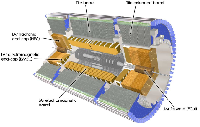
\includegraphics[width=.8\linewidth]{calorimeters}
    \caption{Cut-away view of the ATLAS calorimeter system~\cite{ATLASPaper}.}
    \label{fig:calo}
\end{figure}
%%% Local Variables:
%%% mode: latex
%%% TeX-master: "../search_for_DM_LED_with_ATLAS"
%%% End:
